
\chapter{Inversion method}
\section{Introduction}
The subject of the first laboratory was the so called inverse method.\\
The inverse method is a procedure for obtaining random samples subject to
an invertible cumulative distribution function, given a uniform 
distribution, which is easier to obtain samples from. This is very useful, as most
software used today provides some kind of uniform random variable generator -- some
variation of the rand() function -- which with the inversion method can be
used to generate a set of samples following a different probability distribution.\\
The general procedure goes as follows:
\begin{enumerate}
    \item A desired cumulative distribution $F_x(x) = \int_{-\infty}^{x}f_x(x)dx$ is given
    \item Its inverse $F_x^{-1}(\cdot)$ is calculated
    \item A set of samples $u \sim \mathcal{U}[0,1]$ is generated
    \item By evaluating the inverse at the generated samples, we'll obtain a new set of random variables,
        with $F_x(\cdot)$ as its new cumulative distribution function, e.g.  $F_x^{-1}(u) \sim f_x(\cdot)$
\end{enumerate}
\clearpage
\section{Laboratory}
During the class, we were given a probability density function, from which we were to obtain the cumulative
distribution function, find its inverse, and check if evaluating this inverse at a set of uniformly random samples
gives a set of samples which follow the original density function.
\subsection{Cumulative density function}
The probability density function $f_x(x)$ was given by the equation: 
\begin{equation}
    f_x(x) = \begin{cases}
        0 \text{ for } x < -1\\
       1 + x  \text{ for }  -1 \le x < 0\\
        1 - x \text{ for } 0 \le x < 1\\
        0 \text{ for } x > 1\\
    \end{cases}
\end{equation}
Its integral was given by integrating each piecewise differentiable segment, while keeping in mind that the resulting function may not have any discontinuities. That ultimately gave:
\begin{equation}
    F_x(x) = \begin{cases}
        0 \text{ for } x < -1\\
       \frac{1}{2} + x + \frac{x^{2}}{2}  \text{ for }  -1 \le x < 0\\
      \frac{1}{2} + x - \frac{x^{2}}{2} \text{ for } 0 \le x < 1\\
        1 \text{ for } x > 1\\
    \end{cases}
\end{equation}

\begin{center}
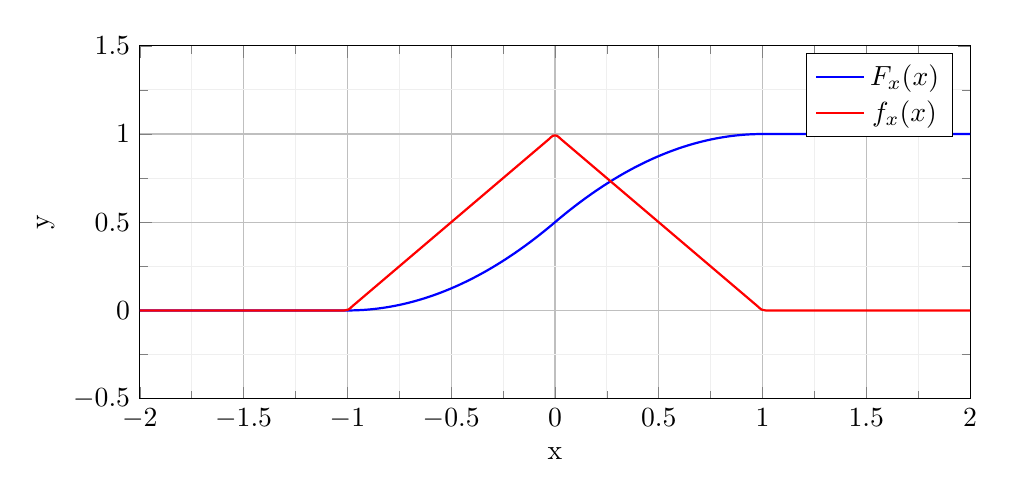
\begin{tikzpicture}
 
\begin{axis}[
    xmin = -2, xmax = 2,
    ymin = -0.5, ymax = 1.5,
    grid = both,
    minor tick num = 1,
    major grid style = {lightgray},
    minor grid style = {lightgray!25},
    width = \textwidth,
    height = 0.5\textwidth,
    xlabel = x,
    ylabel = y]
    \addplot[
        domain = -2:2,
        samples = 200,
        smooth,
        thick,
        blue,
        ] 
        {
        (x < -1)*(0) +
        (x > -1)*(x < 0)*( 0.5 +x + 0.5*x^2) +
        (x > 0)*(x < 1)*( 0.5 + x - 0.5*x^2) +
        (x > 1)*(1)
        };


    \addplot[
        domain = -2:2,
        samples = 200,
        smooth,
        thick,
        red,
        ] 
        {
        (x < -1)*(0) +
        (x > -1)*(x < 0)*(1 + x) +
        (x > 0)*(x < 1)*( 1 - x) +
        (x > 1)*(0)
        };

    \legend{$F_x(x)$,
            $f_x(x)$}
\end{axis}
 
\end{tikzpicture}
\end{center}

\subsection{Inverse cumulative density function}
To get the inverse of the distribution function the equation $u = F_x(x)$ had to be solved for x at each interval giving:
\begin{equation}
   F_x^{-1}(u) = \begin{cases}
       \sqrt{2u} - 1 \text{ for }  0 \le u < \frac{1}{2}\\
       1 - \sqrt{2-2u}\text{ for } \frac{1}{2} \le u < 1\\
    \end{cases}
\end{equation}
2 intervals were lost, as on these intervals the function wasn't bijective and as such, its inverse didn't exist.

\begin{center}
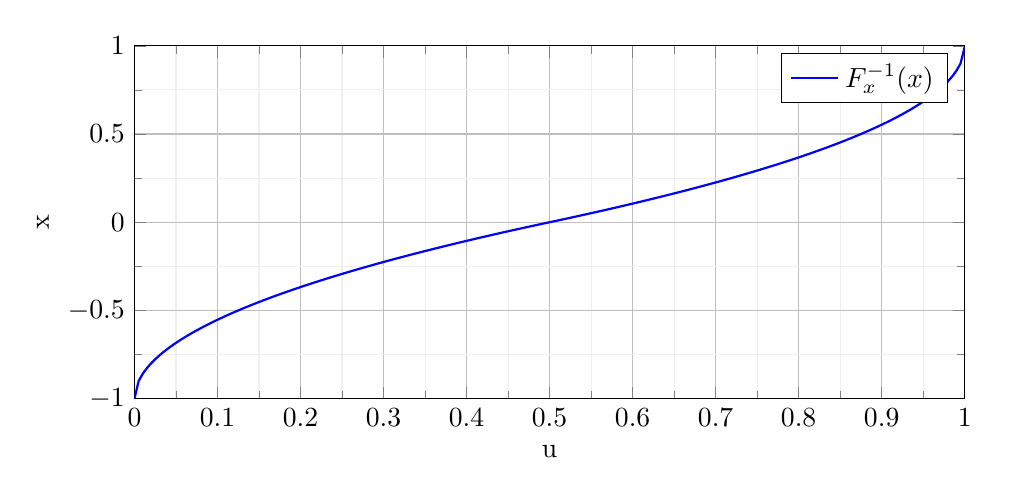
\begin{tikzpicture}
 
\begin{axis}[
    xmin = 0, xmax = 1,
    ymin = -1, ymax = 1,
    grid = both,
    minor tick num = 1,
    major grid style = {lightgray},
    minor grid style = {lightgray!25},
    width = \textwidth,
    height = 0.5\textwidth,
    xlabel = u,
    ylabel = x]


    \addplot[
        domain = 0:1,
        samples = 200,
        %smooth,
        thick,
        blue,
        ] 
        {(x < (0.5))*(x >= 0)*( sqrt(2*x) - 1 ) + 
        (x < 1)*(x >= 0.5)*(1- sqrt(2-2*x)  )
        };
    \legend{$F_x^{-1}(x)$}


\end{axis}
 
\end{tikzpicture}
\end{center}

\subsection{Generating samples following $f_x(x)$}
A set of uniform samples $u\sim \mathcal{U}[0,1]$ were generated, and used as arguments for $F_x^{-1(\cdot)}$. The resulting set of random variables was plotted using a histogram with 50 bins in matlab, giving the following figure as the result:
%%%

\begin{figure}[h!]
    \begin{center}
    \fbox{\includegraphics[clip, trim = 4cm 8cm 4cm 8cm, scale =0.75]{lab1_hist.pdf}}
    \caption{Obtained triangle density function histogram}
    \end{center}
\end{figure}



Clearly, the resulting set follows the desired probability density function, and was generated using only a uniform generator, showing the usefulness of the method.

\clearpage

\chapter{Rejection method}
\section{Introduction}
Despite the usefulness of the inversion method, it has the significant drawback of needing to find the inverse of the cumulative distribution function. Because this function is non-decreasing, there is always an interval where this is in theory possible, it may however be impossible to find analytic expressions for them. The rejection method is a more general procedure for obtaining random variables following a given probability density function only using a known generator, and specifying the desired probability density function.\\
Given a random number generator, which generates random variables according to a probability density function $g(x)$, and a desired density function $f(x)$, such that $ \exists c  \in \mathbb{R}\: \forall \:x f(x) \le cg(x)$, the general procedure works as follows:
\begin{enumerate}
    \item Generate $x \sim g(x)$ and  $u \sim \mathcal{U}[0,1]$
    \item  Build pairs $(x,cg(x)u)$
    \item If $cg(x)u \le f(x)$ keep x in the set, otherwise reject it
\end{enumerate}
As the name suggests, we reject those values of x, which if kept would disturb the probability density function away from the desired one. Of note is that  $g(x)$ can be generated with the inverse method if the uniform distribution by itself is not sufficient. Something to also keep in mind is that if $f(x)$ is not compactly supported,  $g(x)$ will also have to be not compactly supported. If however  $f(x)$ is compactly supported,  $g(x)$ can be not compactly supported, but many more samples may be required to obtain the desired distribution in the resulting set.
\section{Laboratory}
During the laboratory, we were tasked with generating a set of random variables, who's probability density function would be $\sqrt{\frac{2}{\pi}-x^2}$, the upper half of a circle of area 2.
\subsection{Choosing $g(x)$ and $c$}
Since $f(x)$ is compactly supported, the easiest choice for $g(x)$ was a shifted and rescaled uniform distribution:
\begin{equation}
   g(x) = \begin{cases}
       0 \text{ for } x \le - \sqrt{\frac{2}{\pi}}\\
       \frac{1}{2\sqrt{\frac{2}{\pi}}} \text{ for } -\sqrt{\frac{2}{\pi}} < x \le \sqrt{\frac{2}{\pi}}\\
       0 \text{ for } x > \sqrt{\frac{2}{\pi}}\\
    \end{cases}
\end{equation}
Obtaining such distribution is a simple exercise in using the inverse method
giving $x = 2\sqrt{\frac{2}{\pi}}u - \sqrt{\frac{2}{\pi}}$, where $u \sim \mathcal{U}[0,1]$. The value of $c$ can be arbitrary, the best results -- smallest number of samples rejected -- are given by choosing smallest possible c. In this case it means, that  $g(x)*c \le \max{g(x)} = \sqrt{\frac{2}{\pi}}$, which gives $c = \frac{4}{\pi}$.


\begin{center}
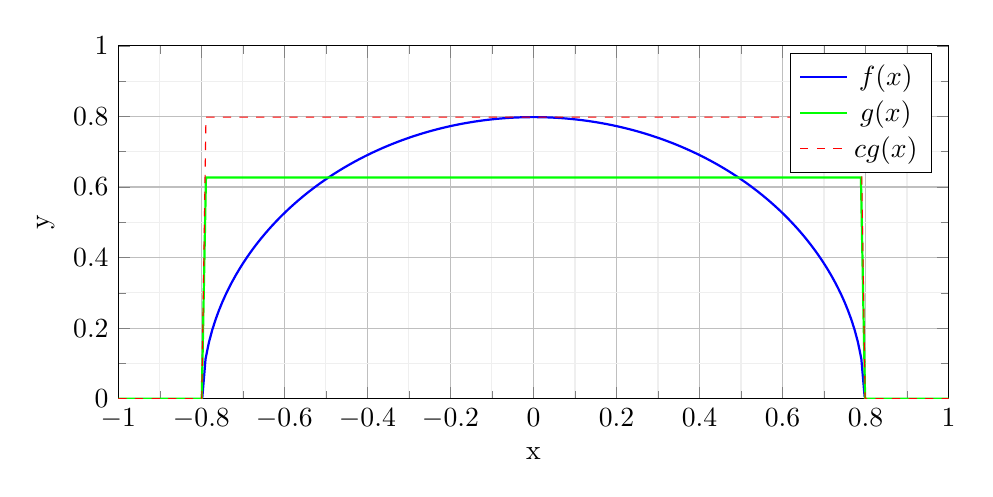
\begin{tikzpicture}
 
\begin{axis}[
    xmin = -1, xmax = 1,
    ymin = 0, ymax = 1,
    grid = both,
    minor tick num = 1,
    major grid style = {lightgray},
    minor grid style = {lightgray!25},
    width = \textwidth,
    height = 0.5\textwidth,
    xlabel = x,
    ylabel = y]


    \addplot[
        domain = (-sqrt(2/3.1415)):(sqrt(2/3.1415)),
        samples = 200,
        %smooth,
        thick,
        blue,
        ] 
        {
            sqrt(2/3.1415-x^2)
        };

    \addplot[
        domain = -1:1,
        samples = 200,
        %smooth,
        thick,
        green,
        ] 
        {
         (x > (-sqrt(2/3.1415)))*(x < (sqrt(2/3.1415))) * (1 / (2*sqrt(2 / 3.1415))) + 0
        };

    \addplot[
        domain = -1:1,
        samples = 200,
        %smooth,
        dashed,
        red,
        ] 
        {
         (x > (-sqrt(2/3.1415)))*(x < (sqrt(2/3.1415))) *(sqrt(2 / 3.1415)) + 0
        };

    \legend{$f(x)$,
            $g(x)$,
            $cg(x)$}

\end{axis}
\end{tikzpicture}
\end{center}

\subsection{Results}
A matlab program was written to generate the pairs in step 2 of the procedure, as well as reject the unneeded samples. The results were plotted as a 50 bin histogram seen in the figure below:
%%\\
\\

\begin{figure}[h!]
    \begin{center}
    \fbox{\includegraphics[clip, trim = 4cm 8cm 4cm 8cm, scale =0.75]{lab2_hist.pdf}}

    \caption{Resulting plots}
    \end{center}
\end{figure}




These results demonstrate, that armed with both the inverse, and the rejection method, one can easily obtain sets of random variables following arbitrary distributions fairly easily.

